\documentclass[12pt,
brazilian,
a5paper]{abntex2} % Default font size and left-justified equations

%%%%%%%%%%%%%%%%%%%%%%%%%%%%%%%%%%%%%%%%%
% The Legrand Orange Book
% Structural Definitions File
% Version 2.1 (26/09/2018)
%
% Original author:
% Mathias Legrand (legrand.mathias@gmail.com) with modifications by:
% Vel (vel@latextemplates.com)
%
% This file was downloaded from:
% http://www.LaTeXTemplates.com
%
% License:
% CC BY-NC-SA 3.0 (http://creativecommons.org/licenses/by-nc-sa/3.0/)
%
%%%%%%%%%%%%%%%%%%%%%%%%%%%%%%%%%%%%%%%%%

% % ----------------------------------------------------------------------------------------
% %	VARIOUS REQUIRED PACKAGES AND CONFIGURATIONS
% % ----------------------------------------------------------------------------------------

% \hypersetup{pdftitle={Title},pdfauthor={Author}} % Uncomment and fill out to include PDF metadata for the author and title of the book

% \usepackage{mathtools}
% \usepackage{amsfonts}
% \usepackage{mathrsfs} % para mathscr

\usepackage{ifxetex}
\ifxetex
% % se for utilizar as fontes do sistema: **escolha sua fonte**
% comandos de fontes
\usepackage{mathspec}
\setmathsfont(Digits,Latin,Greek){Minion Pro}
\setmathrm{Minion Pro}
\setmainfont[Numbers=OldStyle]{Minion Pro} %fonte principal (serifada)
\setsansfont[Scale=0.9]{Myriad Pro} %fonte sem serifas
\setmonofont[Scale=MatchLowercase]{Consolas} % fonte monoespaçada

\usepackage{polyglossia} %always load polyblossia after fonts for digits in math mode
\setmainlanguage{brazil}
\setotherlanguages{french,english,spanish,german,italian}

\else
% % se for utilizar pdflatex
% \usepackage[utf8]{inputenc}
% \usepackage{newtxmath}
% \usepackage{Alegreya}
% \usepackage{AlegreyaSans}
\usepackage[nf]{coelacanth}
\usepackage[T1]{fontenc}
%% The font package uses mweights.sty which has som issues with the
%% \normalfont command. The following two lines fixes this issue.
\let\oldnormalfont\normalfont
\def\normalfont{\oldnormalfont\mdseries}
\usepackage[lf]{FiraMono}
\usepackage[italic]{mathastext}
\usepackage{slantsc}
\fi


%% Observação: o pacote polyglossia pode apresentar erro ao ser utilizado com ifxetex + babel.
%% Se isso acontecer, atualize o pacote para a versão mais recente ou utilize somente uma das sequências (pdflatex ou xelatex), comentando ou apagando a outra.

\usepackage{microtype} 				% para melhorias de justificação
% \usepackage[dvipsnames]{xcolor} 		% para cores
% \usepackage{graphicx} 			% para imagens
\usepackage{booktabs,tabularx,rotating}	% para tabelas
\usepackage{mdframed} 				% para caixas de texto como na CIP do verso do título
\usepackage{multicol}				% tabelas com colunas mescladas
\usepackage{lettrine}				% letras capitulares
\usepackage{xspace} 				% para nao precisar de espaços com {} depois de comandos
% como \LaTeX e abreviações criadas pelo usuário
\usepackage{lipsum} 				% para texto de preenchimento de exemplo
\usepackage{leading}				% espaçamento entrelinhas (leading)
\leading{13pt}

% ---
% Pacotes de citações
% ---
\usepackage[brazilian,hyperpageref]{backref}	 % Paginas com as citações na bibl
\usepackage[alf]{abntex2cite}	% Citações padrão ABNT

% ---
% Configurações do pacote backref
% Usado sem a opção hyperpageref de backref
\renewcommand{\backrefpagesname}{Citado na(s) página(s):~}
% Texto padrão antes do número das páginas
\renewcommand{\backref}{}
% Define os textos da citação
\renewcommand*{\backrefalt}[4]{
  \ifcase #1 %
  Nenhuma citação no texto.%
  \or
  Citado na página #2.%
  \else
  Citado #1 vezes nas páginas #2.%
  \fi}%
% ---


%% Spacing of general text; among lines, chapter, section etc
\setlength{\parindent}{1.3em}
\setlength{\parskip}{0.2em}
\renewcommand{\baselinestretch}{1.0}


\usepackage{graphicx} % Required for including pictures
\graphicspath{{Pictures/}} % Specifies the directory where pictures are stored

\usepackage{lipsum} % Inserts dummy text

\usepackage[edges]{forest}    %%Hierarchy Diagram
\usetikzlibrary{shadows.blur}

\usepackage{tikz} % Required for drawing custom shapes

% \usepackage[brazilian]{babel} % English language/hyphenation

\usepackage{enumitem} % Customize lists
\setlist{nolistsep} % Reduce spacing between bullet points and numbered lists

\usepackage{booktabs} % Required for nicer horizontal rules in tables

\usepackage{xcolor} % Required for specifying colors by name
\definecolor{ocre}{RGB}{243,102,25} % Define the orange color used for highlighting throughout the book

% % \usepackage{abntex2}

% % ----------------------------------------------------------------------------------------
% %	MARGINS
% % ----------------------------------------------------------------------------------------

\usepackage{geometry} % Required for adjusting page dimensions and margins

\geometry{
  paper=a4paper, % Paper size, change to letterpaper for US letter size
  top=2cm, % Top margin
  bottom=2cm, % Bottom margin
  left=2.3cm, % Left margin
  right=2.3cm, % Right margin
  headheight=3pt, % Header height
  footskip=1.5cm, % Space from the bottom margin to the baseline of the footer
  headsep=1cm, % Space from the top margin to the baseline of the header
  % showframe, % Uncomment to show how the type block is set on the page
}

% % ----------------------------------------------------------------------------------------
% %	FONTS
% % ----------------------------------------------------------------------------------------

% \usepackage{lmodern}	% Usa a fonte Latin Modern
% \usepackage{avant} % Use the Avantgarde font for headings
% % \usepackage{times} % Use the Times font for headings
% \usepackage{mathptmx} % Use the Adobe Times Roman as the default text font together with math symbols from the Sym­bol, Chancery and Com­puter Modern fonts

% \usepackage{microtype} % Slightly tweak font spacing for aesthetics
% \usepackage[utf8]{inputenc} % Required for including letters with accents
% \usepackage[T1]{fontenc} % Use 8-bit encoding that has 256 glyphs
\usepackage{indentfirst}		% Indenta o primeiro parágrafo de cada seção.

% % ----------------------------------------------------------------------------------------
% %	BIBLIOGRAPHY AND INDEX
% % ----------------------------------------------------------------------------------------

% \usepackage[style=numeric,citestyle=numeric,sorting=nyt,sortcites=true,autopunct=true,babel=hyphen,hyperref=true,abbreviate=false,backref=true,backend=biber]{biblatex}
% \addbibresource{bibliography} % BibTeX bibliography file
% \defbibheading{bibempty}{}

% ---
% Pacotes de citações
% ---
\usepackage[brazilian,hyperpageref]{backref}	 % Paginas com as citações na bibl
\usepackage[alf]{abntex2cite}	% Citações padrão ABNT
\usepackage{abntex2abrev}
% ---
% CONFIGURAÇÕES DE PACOTES
% ---

% ---
% Configurações do pacote backref
% Usado sem a opção hyperpageref de backref
\renewcommand{\backrefpagesname}{Citado na(s) página(s):~}
% Texto padrão antes do número das páginas
\renewcommand{\backref}{}
% Define os textos da citação
\renewcommand*{\backrefalt}[4]{
  \ifcase #1 %
  Nenhuma citação no texto.%
  \or
  Citado na página #2.%
  \else
  Citado #1 vezes nas páginas #2.%
  \fi}%
% ---

\usepackage{calc} % For simpler calculation - used for spacing the index letter headings correctly
\usepackage{makeidx} % Required to make an index
\makeindex % Tells LaTeX to create the files required for indexing

% ----------------------------------------------------------------------------------------
%	MAIN TABLE OF CONTENTS
% ----------------------------------------------------------------------------------------

\usepackage{titletoc} % Required for manipulating the table of contents

\contentsmargin{0cm} % Removes the default margin

% Part text styling (this is mostly taken care of in the PART HEADINGS section of this file)
\titlecontents{part}
[0cm] % Left indentation
{\addvspace{13pt}\bfseries} % Spacing and font options for parts
{}
{}
{}

% Chapter text styling
\titlecontents{chapter}
[1.25cm] % Left indentation
{\addvspace{20pt}\large\sffamily\bfseries} % Spacing and font options for chapters
{\color{ocre!60}\contentslabel[\Large\thecontentslabel]{1.5cm}\color{ocre}} % Formatting of numbered sections of this type
{\color{ocre}} % Formatting of numberless sections of this type
{\color{ocre!60}\normalsize\;\titlerule*[.5pc]{.}\;\thecontentspage}

% Formatting of the filler to the right of the heading and the
% page number

% Section text styling
\titlecontents{section}
[1.25cm] % Left indentation
{\addvspace{1pt}\sffamily\bfseries} % Spacing and font options for sections
{\contentslabel[\thecontentslabel]{1.25cm}} % Formatting of numbered sections of this type
{} % Formatting of numberless sections of this type
{\hfill\color{black}\thecontentspage} % Formatting of the filler to the right of the heading and the page number

% Subsection text styling
\titlecontents{subsection}
[1.25cm] % Left indentation
{\addvspace{1pt}\sffamily\small} % Spacing and font options for subsections
{\contentslabel[\thecontentslabel]{1.25cm}} % Formatting of numbered sections of this type
{} % Formatting of numberless sections of this type
{\ \titlerule*[.5pc]{.}\;\thecontentspage} % Formatting of the filler to the right of the heading and the page number

% Figure text styling
\titlecontents{figure}
[1.25cm] % Left indentation
{\addvspace{1pt}\sffamily\small} % Spacing and font options for figures
{\thecontentslabel\hspace*{1em}} % Formatting of numbered sections of this type
{} % Formatting of numberless sections of this type
{\ \titlerule*[.5pc]{.}\;\thecontentspage} % Formatting of the filler to the right of the heading and the page number

% Table text styling
\titlecontents{table}
[1.25cm] % Left indentation
{\addvspace{1pt}\sffamily\small} % Spacing and font options for tables
{\thecontentslabel\hspace*{1em}} % Formatting of numbered sections of this type
{} % Formatting of numberless sections of this type
{\ \titlerule*[.5pc]{.}\;\thecontentspage} % Formatting of the filler to the right of the heading and the page number

% ----------------------------------------------------------------------------------------
%	MINI TABLE OF CONTENTS IN PART HEADS
% ----------------------------------------------------------------------------------------

% Chapter text styling
\titlecontents{lchapter}
[0em] % Left indentation
{\addvspace{15pt}\large\sffamily\bfseries} % Spacing and font options for chapters
{\color{ocre}\contentslabel[\Large\thecontentslabel]{1.25cm}\color{ocre}} % Chapter number
{}
{\color{ocre}\normalsize\sffamily\bfseries\;\titlerule*[.5pc]{.}\;\thecontentspage} % Page number

% % Section text styling
\titlecontents{lsection}
[0em] % Left indentation
{\sffamily\small} % Spacing and font options for sections
{\contentslabel[\thecontentslabel]{1.25cm}} % Section number
{}
{}

% Subsection text styling (note these aren't shown by default, display them by searchings this file for tocdepth and reading the commented text)
\titlecontents{lsubsection}
[.5em] % Left indentation
{\sffamily\footnotesize} % Spacing and font options for subsections
{\contentslabel[\thecontentslabel]{1.25cm}}
{}
{}

% ----------------------------------------------------------------------------------------
%	HEADERS AND FOOTERS
% ----------------------------------------------------------------------------------------

\usepackage{fancyhdr} % Required for header and footer configuration

\pagestyle{fancy} % Enable the custom headers and footers

\renewcommand{\chaptermark}[1]{\markboth{\sffamily\large\bfseries\chaptername\
    \thechapter.\ #1}{}} % Styling for the current chapter in the header
\renewcommand{\sectionmark}[1]{\markright{\sffamily\large\thesection\hspace{2pt}#1}{}} % Styling for the current section in the header

\fancyhf{} % Clear default headers and footers
\fancyhead[LE,RO]{\sffamily\large\thepage} % Styling for the page number in the header
\fancyhead[LO]{\rightmark} % Print the nearest section name on the left side of odd pages
\fancyhead[RE]{\leftmark} % Print the current chapter name on the right side of even pages
\fancyfoot[C]{\thepage} % Uncomment to include a footer

\renewcommand{\headrulewidth}{0.8pt} % Thickness of the rule under the header

\fancypagestyle{plain}{% Style for when a plain pagestyle is specified
  \fancyhead{}\renewcommand{\headrulewidth}{0pt}%
}

% Removes the header from odd empty pages at the end of chapters
\makeatletter
\renewcommand{\cleardoublepage}{
  \clearpage\ifodd\c@page\else
  \hbox{}
  \vspace*{\fill}
  \thispagestyle{empty}
  \newpage
  \fi}

% ----------------------------------------------------------------------------------------
%	THEOREM STYLES
% ----------------------------------------------------------------------------------------

\usepackage{amsmath,amsfonts,amssymb,amsthm} % For math equations, theorems, symbols, etc

\newcommand{\intoo}[2]{\mathopen{]}#1\,;#2\mathclose{[}}
\newcommand{\ud}{\mathop{\mathrm{{}d}}\mathopen{}}
\newcommand{\intff}[2]{\mathopen{[}#1\,;#2\mathclose{]}}
\renewcommand{\qedsymbol}{$\blacksquare$}
\newtheorem{notation}{Notation}[chapter]

% Boxed/framed environments
\newtheoremstyle{ocrenumbox}% Theorem style name
{0pt}% Space above
{0pt}% Space below
{\normalfont}% Body font
{}% Indent amount
{\small\bf\sffamily\color{ocre}}% Theorem head font
{\;}% Punctuation after theorem head
{0.25em}% Space after theorem head
{\small\sffamily\color{ocre}\thmname{#1}\nobreakspace\thmnumber{\@ifnotempty{#1}{}\@upn{#2}}% Theorem text (e.g. Theorem 2.1)
  \thmnote{\nobreakspace\the\thm@notefont\sffamily\bfseries\color{black}---\nobreakspace#3.}} % Optional theorem note

\newtheoremstyle{blacknumex}% Theorem style name
{5pt}% Space above
{5pt}% Space below
{\normalfont}% Body font
{} % Indent amount
{\small\bf\sffamily}% Theorem head font
{\;}% Punctuation after theorem head
{0.25em}% Space after theorem head
{\small\sffamily{\tiny\ensuremath{\blacksquare}}\nobreakspace\thmname{#1}\nobreakspace\thmnumber{\@ifnotempty{#1}{}\@upn{#2}}% Theorem text (e.g. Theorem 2.1)
  \thmnote{\nobreakspace\the\thm@notefont\sffamily\bfseries---\nobreakspace#3.}}% Optional theorem note

\newtheoremstyle{blacknumbox} % Theorem style name
{0pt}% Space above
{0pt}% Space below
{\normalfont}% Body font
{}% Indent amount
{\small\bf\sffamily}% Theorem head font
{\;}% Punctuation after theorem head
{0.25em}% Space after theorem head
{\small\sffamily\thmname{#1}\nobreakspace\thmnumber{\@ifnotempty{#1}{}\@upn{#2}}% Theorem text (e.g. Theorem 2.1)
  \thmnote{\nobreakspace\the\thm@notefont\sffamily\bfseries---\nobreakspace#3.}}% Optional theorem note

% Non-boxed/non-framed environments
\newtheoremstyle{ocrenum}% Theorem style name
{5pt}% Space above
{5pt}% Space below
{\normalfont}% Body font
{}% Indent amount
{\small\bf\sffamily\color{ocre}}% Theorem head font
{\;}% Punctuation after theorem head
{0.25em}% Space after theorem head
{\small\sffamily\color{ocre}\thmname{#1}\nobreakspace\thmnumber{\@ifnotempty{#1}{}\@upn{#2}}% Theorem text (e.g. Theorem 2.1)
  \thmnote{\nobreakspace\the\thm@notefont\sffamily\bfseries\color{black}---\nobreakspace#3.}} % Optional theorem note
\makeatother

% Defines the theorem text style for each type of theorem to one of the three styles above
\newcounter{dummy}
\numberwithin{dummy}{section}
\theoremstyle{ocrenumbox}
\newtheorem{theoremeT}[dummy]{Theorem}
\newtheorem{problem}{Problem}[chapter]
\newtheorem{exerciseT}{Exercise}[chapter]
\theoremstyle{blacknumex}
\newtheorem{exampleT}{Example}[chapter]
\theoremstyle{blacknumbox}
\newtheorem{vocabulary}{Vocabulary}[chapter]
\newtheorem{definitionT}{Definition}[section]
\newtheorem{corollaryT}[dummy]{Corollary}
\theoremstyle{ocrenum}
\newtheorem{proposition}[dummy]{Proposition}

% ----------------------------------------------------------------------------------------
%	DEFINITION OF COLORED BOXES
% ----------------------------------------------------------------------------------------

\RequirePackage[framemethod=default]{mdframed} % Required for creating the theorem, definition, exercise and corollary boxes
% Theorem box
\newmdenv[skipabove=7pt,
skipbelow=7pt,
backgroundcolor=black!5,
linecolor=ocre,
innerleftmargin=5pt,
innerrightmargin=5pt,
innertopmargin=5pt,
leftmargin=0cm,
rightmargin=0cm,
innerbottommargin=5pt]{tBox}

% Exercise box
\newmdenv[skipabove=7pt,
skipbelow=7pt,
rightline=false,
leftline=true,
topline=false,
bottomline=false,
backgroundcolor=ocre!10,
linecolor=ocre,
innerleftmargin=5pt,
innerrightmargin=5pt,
innertopmargin=5pt,
innerbottommargin=5pt,
leftmargin=0cm,
rightmargin=0cm,
linewidth=4pt]{eBox}

% Definition box
\newmdenv[skipabove=7pt,
skipbelow=7pt,
rightline=false,
leftline=true,
topline=false,
bottomline=false,
linecolor=ocre,
innerleftmargin=5pt,
innerrightmargin=5pt,
innertopmargin=0pt,
leftmargin=0cm,
rightmargin=0cm,
linewidth=4pt,
innerbottommargin=0pt]{dBox}

% Corollary box
\newmdenv[skipabove=7pt,
skipbelow=7pt,
rightline=false,
leftline=true,
topline=false,
bottomline=false,
linecolor=gray,
backgroundcolor=black!5,
innerleftmargin=5pt,
innerrightmargin=5pt,
innertopmargin=5pt,
leftmargin=0cm,
rightmargin=0cm,
linewidth=4pt,
innerbottommargin=5pt]{cBox}

% Creates an environment for each type of theorem and assigns it a theorem text style from the "Theorem Styles" section above and a colored box from above
\newenvironment{theorem}{\begin{tBox}\begin{theoremeT}}{\end{theoremeT}\end{tBox}}
\newenvironment{exercise}{\begin{eBox}\begin{exerciseT}}{\hfill{\color{ocre}\tiny\ensuremath{\blacksquare}}\end{exerciseT}\end{eBox}}
\newenvironment{definition}{\begin{dBox}\begin{definitionT}}{\end{definitionT}\end{dBox}}
\newenvironment{example}{\begin{exampleT}}{\hfill{\tiny\ensuremath{\blacksquare}}\end{exampleT}}
\newenvironment{corollary}{\begin{cBox}\begin{corollaryT}}{\end{corollaryT}\end{cBox}}

% ----------------------------------------------------------------------------------------
%	REMARK ENVIRONMENT
% ----------------------------------------------------------------------------------------

\newenvironment{remark}{%\par\vspace{10pt}\small % Vertical white space above the remark and smaller font size
  \begin{list}{}{
      \leftmargin=20pt % Indentation on the left
      \rightmargin=25pt}\item\ignorespaces % Indentation on the right
    \makebox[-2.5pt]{\begin{tikzpicture}[overlay]
        \node[draw=ocre!60,line width=1pt,circle,fill=ocre!25,font=\sffamily\bfseries,inner sep=2pt,outer sep=0pt] at (-15pt,0pt){\textcolor{ocre}{R}};\end{tikzpicture}} % Orange R in a circle
    \advance\baselineskip -1pt}{\end{list}\vskip5pt} % Tighter line spacing and white space after remark

% ----------------------------------------------------------------------------------------
%	SECTION NUMBERING IN THE MARGIN
% ----------------------------------------------------------------------------------------

\makeatletter
\renewcommand{\@seccntformat}[1]{\llap{\textcolor{ocre}{\csname the#1\endcsname}\hspace{1em}}}
\renewcommand{\section}{\@startsection{section}{1}{\z@}
  {-4ex \@plus -1ex \@minus -.4ex}
  {1ex \@plus.2ex }
  {\Large\scfamily\bfseries}}
\renewcommand{\subsection}{\@startsection {subsection}{2}{\z@}
  {-3ex \@plus -0.1ex \@minus -.4ex}
  {0.5ex \@plus.2ex }
  {\large\scfamily\bfseries}}
\renewcommand{\subsubsection}{\@startsection {subsubsection}{3}{\z@}
  {-2ex \@plus -0.1ex \@minus -.2ex}
  {.2ex \@plus.2ex }
  {\normalfont\large\scfamily\bfseries}}
\renewcommand\paragraph{\@startsection{paragraph}{4}{\z@}
  {-2ex \@plus-.2ex \@minus .2ex}
  {.1ex}
  {\normalfont\large\sffamily\bfseries}}

% ----------------------------------------------------------------------------------------
%	PART HEADINGS
% ----------------------------------------------------------------------------------------

% Numbered part in the table of contents
\newcommand{\@mypartnumtocformat}[2]{%
  \setlength\fboxsep{0pt}%
  \noindent\colorbox{ocre!20}{\strut\parbox[c][.7cm]{\ecart}{\color{ocre!70}\Large\sffamily\bfseries\centering#1}}\hskip\esp\colorbox{ocre!40}{\strut\parbox[c][0.7cm]{\linewidth-\ecart-\esp}{\Large\sffamily\centering#2}}%
}

% Unnumbered part in the table of contents
\newcommand{\@myparttocformat}[1]{%
  \setlength\fboxsep{4pt}%
  \noindent\colorbox{ocre!40}{\strut\parbox[c][0.7cm]{\linewidth}{\Large\sffamily\centering#1}}%
}

\newlength\esp
\setlength\esp{2pt}
\newlength\ecart
\setlength\ecart{0.2cm-\esp}
\newcommand{\thepartimage}{}%
\newcommand{\partimage}[1]{\renewcommand{\thepartimage}{#1}}%
\def\@part[#1]#2{%
  \ifnum \c@secnumdepth >-2\relax%
  \refstepcounter{part}%
  \addcontentsline{toc}{part}{\texorpdfstring{\protect\@mypartnumtocformat{\thepart}{#1}}{\partname~\thepart\ ---\ #1}}
  \else%
  \addcontentsline{toc}{part}{\texorpdfstring{\protect\@myparttocformat{#1}}{#1}}%
  \fi%
  \startcontents%
  \markboth{}{}%
  {\thispagestyle{empty}%
    \begin{tikzpicture}[remember picture,overlay]%
      \node at (current page.north west){\begin{tikzpicture}[remember picture,overlay]%
          \fill[ocre!20](0cm,0cm) rectangle (\paperwidth,-\paperheight);
          \node[anchor=north] at (4cm,-3.25cm){\color{ocre!60}\fontsize{500}{700}\sffamily\bfseries\thepart};
          \node[anchor=south east] at (\paperwidth-2cm,-\paperheight+1cm){\parbox[][][t]{14cm}{
              \printcontents{a}{0}{\setcounter{tocdepth}{4}}% The depth to which the Part mini table of contents displays headings; 0 for chapters only, 1 for chapters and sections and 2 for chapters, sections and subsections
            }};
          \node[anchor=north east] at
          (\paperwidth-3cm,-3.25cm){\parbox[t][][t]{10cm}{\strut\raggedleft\color{white}\fontsize{40}{50}\ttfamily\bfseries#2}};
          %%Parte structure, font, size
        \end{tikzpicture}};
    \end{tikzpicture}}%
  \@endpart}
\def\@spart#1{%
  \startcontents%
  \phantomsection
  {\thispagestyle{empty}%
    \begin{tikzpicture}[remember picture,overlay]%
      \node at (current page.north west){\begin{tikzpicture}[remember picture,overlay]%
          \fill[ocre!40](5cm,5cm) rectangle (\paperwidth,-\paperheight);
          \node[anchor=north east] at (\paperwidth-1.5cm,-3.25cm){\parbox[t][][t]{15cm}{\strut\raggedleft\color{white}\fontsize{30}{30}\sffamily\bfseries#1}};
        \end{tikzpicture}};
    \end{tikzpicture}}
  \addcontentsline{toc}{part}{\texorpdfstring{%
      \setlength\fboxsep{3pt}%
      \noindent\protect\colorbox{ocre!90}{\strut\protect\parbox[l][2cm]{\linewidth}{\Large\sffamily\protect\centering #1\quad\mbox{}}}}{#1}}%
  \@endpart}
\def\@endpart{\vfil\newpage
  \if@twoside
  \if@openright
  \null
  \thispagestyle{empty}%
  \newpage
  \fi
  \fi
  \if@tempswa
  \twocolumn
  \fi}

% ----------------------------------------------------------------------------------------
%	CHAPTER HEADINGS
% ----------------------------------------------------------------------------------------

% A switch to conditionally include a picture, implemented by Christian Hupfer
\newif\ifusechapterimage
\usechapterimagetrue
\newcommand{\thechapterimage}{}%
\newcommand{\chapterimage}[1]{\ifusechapterimage\renewcommand{\thechapterimage}{#1}\fi}%
\newcommand{\autodot}{.}
\def\@makechapterhead#1{%
  {\parindent \z@ \raggedright \normalfont
    \ifnum \c@secnumdepth >\m@ne
    \if@mainmatter
    \begin{tikzpicture}[remember picture,overlay]
      \node at (current page.north west)
      {\begin{tikzpicture}[remember picture,overlay]
          \node[anchor=north west,inner sep=0pt] at (0,0) {\ifusechapterimage\includegraphics[width=\paperwidth]{\thechapterimage}\fi};
          \draw[anchor=west] (\Gm@lmargin,-9cm) node [line width=2.3pt,rounded corners=15pt,draw=ocre,fill=white,fill opacity=0.7,inner sep=15pt]{\strut\makebox[22cm]{}};
          \draw[anchor=west] (\Gm@lmargin+.3cm,-9cm) node {\Large\sffamily\bfseries\color{black}\thechapter\autodot~#1\strut};
        \end{tikzpicture}};
    \end{tikzpicture}
    \else
    \begin{tikzpicture}[remember picture,overlay]
      \node at (current page.north west)
      {\begin{tikzpicture}[remember picture,overlay]
          \node[anchor=north west,inner sep=0pt] at (0,0) {\ifusechapterimage\includegraphics[width=\paperwidth]{\thechapterimage}\fi};
          \draw[anchor=west] (\Gm@lmargin,-8cm) node [line width=2pt,rounded corners=15pt,draw=ocre,fill=white,fill opacity=0.5,inner sep=15pt]{\strut\makebox[22cm]{}};
          \draw[anchor=west] (\Gm@lmargin+.3cm,-8cm) node {\normalsize\sffamily\bfseries\color{black}#1\strut};
        \end{tikzpicture}};
    \end{tikzpicture}
    \fi\fi\par\vspace*{270\p@}}}

% -------------------------------------------

\def\@makeschapterhead#1{%
  \begin{tikzpicture}[remember picture,overlay]
    \node at (current page.north west)
    {\begin{tikzpicture}[remember picture,overlay]
        \node[anchor=north west,inner sep=0pt] at (0,0) {\ifusechapterimage\includegraphics[width=\paperwidth]{\thechapterimage}\fi};
        \draw[anchor=west] (\Gm@lmargin,-9cm) node [line width=2pt,rounded corners=15pt,draw=ocre,fill=white,fill opacity=0.5,inner sep=15pt]{\strut\makebox[22cm]{}};
        \draw[anchor=west] (\Gm@lmargin+.3cm,-9cm) node {\normalsize\sffamily\bfseries\color{black}#1\strut};
      \end{tikzpicture}};
  \end{tikzpicture}
  \par\vspace*{270\p@}}
\makeatother

% ----------------------------------------------------------------------------------------
%	LINKS
% ----------------------------------------------------------------------------------------

\usepackage{hyperref}
\hypersetup{hidelinks,backref=true,pagebackref=true,hyperindex=true,colorlinks=false,breaklinks=true,urlcolor=ocre,bookmarks=true,bookmarksopen=false}

\usepackage{bookmark}
\bookmarksetup{
  open,
  numbered,
  addtohook={%
    \ifnum\bookmarkget{level}=0 % chapter
    \bookmarksetup{bold}%
    \fi
    \ifnum\bookmarkget{level}=-1 % part
    \bookmarksetup{color=ocre,bold}%
    \fi
  }
}



%% Spaces between Chapter, Section, Subsection etc and subsequent text
\usepackage{titlesec}
\titlespacing*{\section}
{2pt}{2ex plus 1ex minus .2ex}{3ex plus .3ex}
\titlespacing*{\subsection}
{2pt}{2ex plus 1ex minus .2ex}{3ex plus .3ex}

%% Chapter, Section, Subsection etc sizes

%%% Local Variables:
%%% mode: latex
%%% TeX-master: "livro"
%%% End:
 % Insert the commands.tex file which contains the majority of the structure behind the template


%% Identação modular no ambiente 'myparident'
\newlength\mystoreparindent
\newenvironment{myparindent}[1]{%
  \setlength{\mystoreparindent}{\the\parindent}
  \setlength{\parindent}{#1}
}{%
  \setlength{\parindent}{\mystoreparindent}
}

\usepackage{verbatimbox}
\usepackage{array}


% ----------------------------------------------------------------------------------------

\begin{document}

% ----------------------------------------------------------------------------------------
%	TITLE PAGE
% ----------------------------------------------------------------------------------------

\begingroup
\thispagestyle{empty} % Suppress headers and footers on the title page
\begin{tikzpicture}[remember picture,overlay]
  \coordinate [below=50cm] (midpoint) at (current page.north);
  \node[inner sep=0pt] (background) at (current page.center) {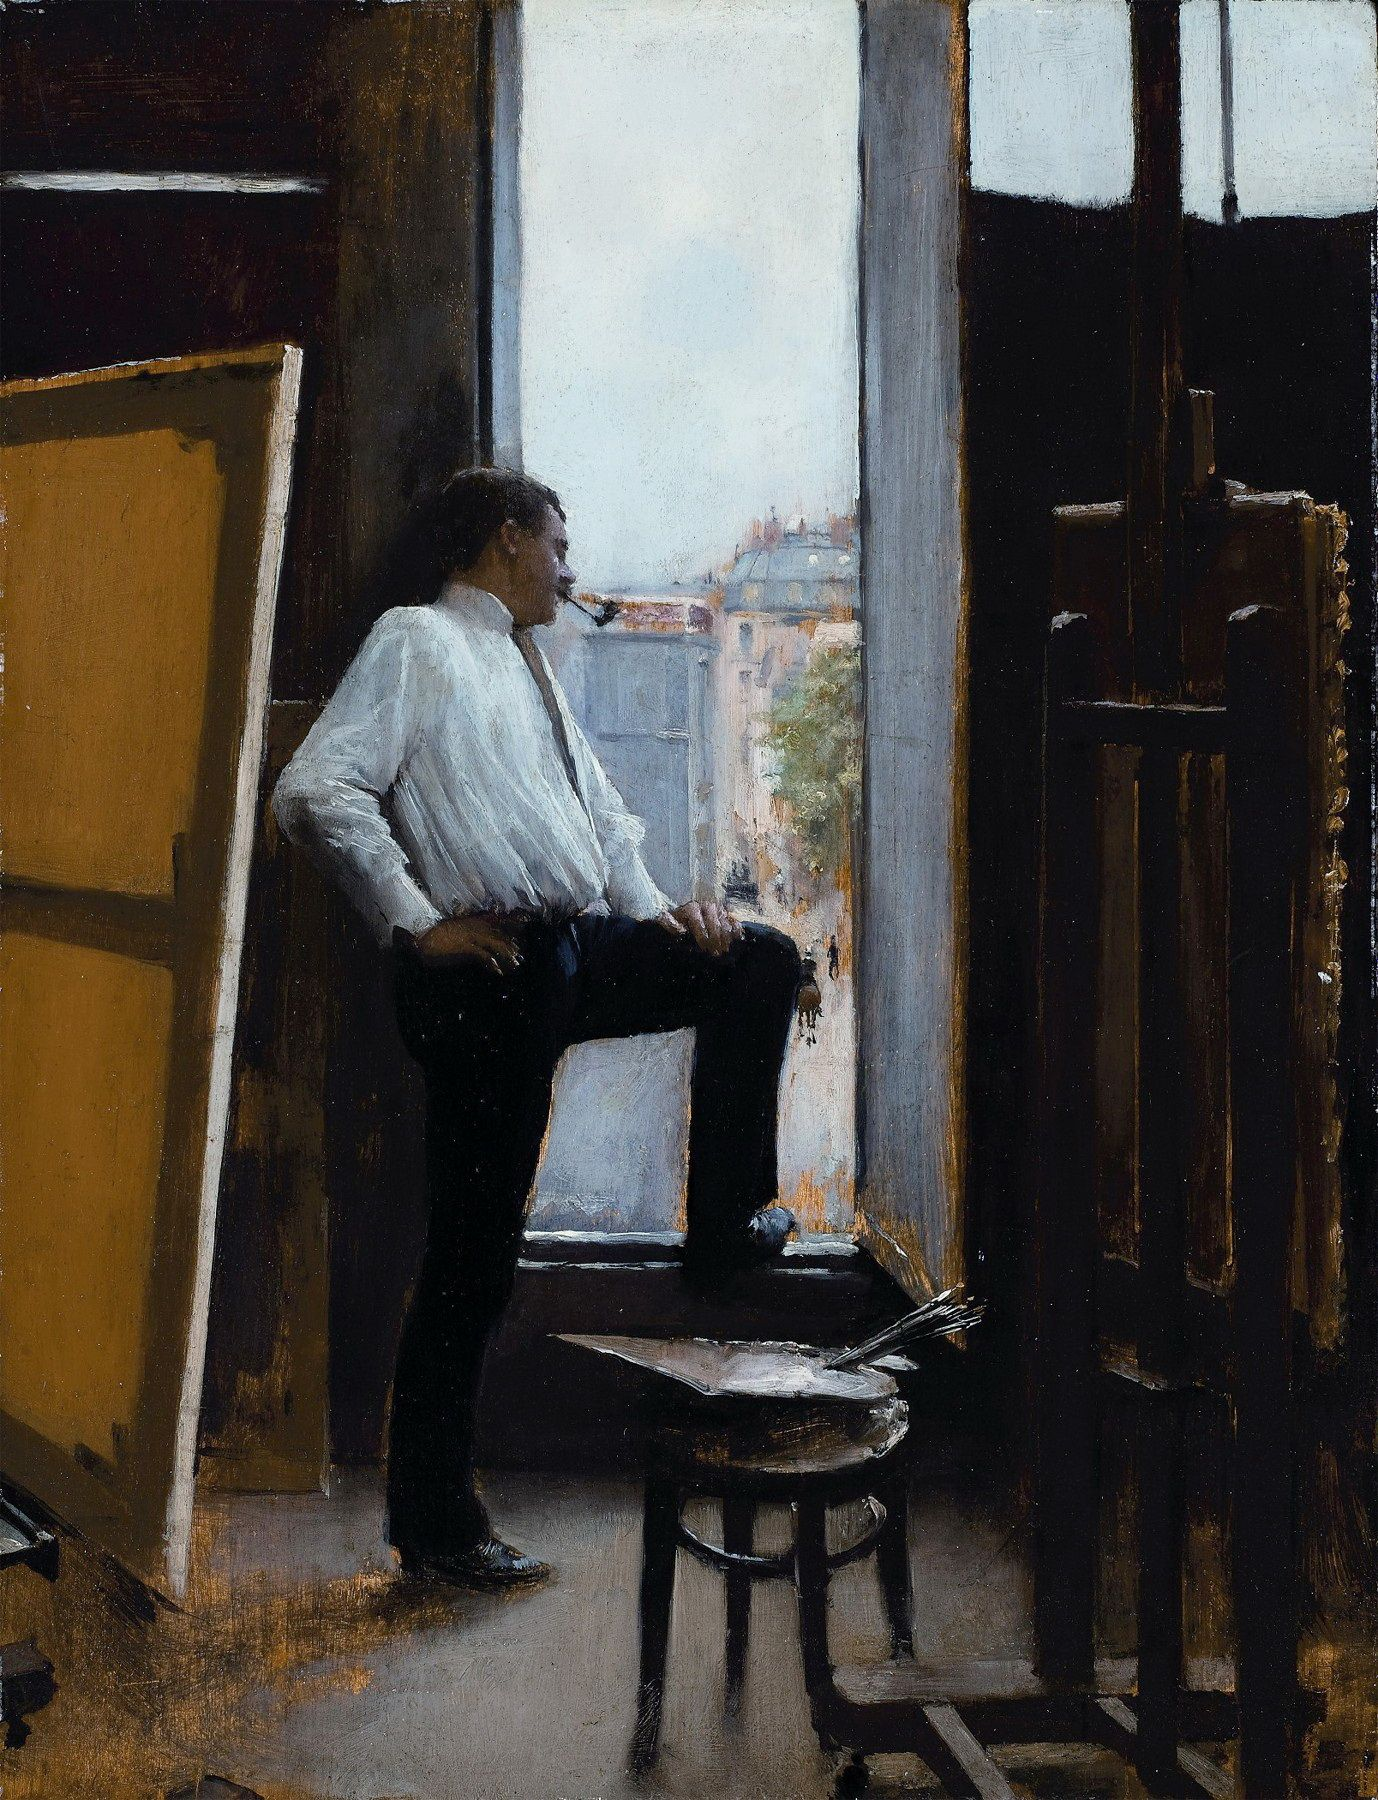
\includegraphics[width=\paperheight]{p21.jpg}};
  \draw (current page.center) node [fill=ocre!50!white,fill
  opacity=0.75,text opacity=2,inner
  sep=1cm]{\Huge\centering\bfseries\rmfamily \color{grey!80!white} \parbox[c][][t]{\paperheight}{\centering
      {\huge  Referências Cruzadas, \\ Apresentações e \\ Sumário dos Comandos Essenciais} \\[20pt] % Book title
      {\Large Parte 3}\\[20pt] % Subtitle
      {\huge Aluno, Pedro G. Branquinho \\ Orientadora, Katia C. G. Candioto}}}; % Author name
\end{tikzpicture}
\vfill
\endgroup


% ----------------------------------------------------------------------------------------
%	COPYRIGHT PAGE
% ----------------------------------------------------------------------------------------

\newpage
~\vfill
\thispagestyle{empty}

\noindent Copyright \copyright\ 2020 Pedro G. Branquinho\\ % Copyright notice

% \noindent \textsc{Published by BuddhiLWinc.}\\ % Publisher

\noindent \textsc{https://github.com/26-55-87-BuddhiLW/MC-LaTeX}\\ % URL

\noindent Licensed under the Creative Commons Attribution-NonCommercial 3.0 Unported License (the ``License''). You may not use this file except in compliance with the License. You may obtain a copy of the License at \url{http://creativecommons.org/licenses/by-nc/3.0}. Unless required by applicable law or agreed to in writing, software distributed under the License is distributed on an \textsc{``as is'' basis, without warranties or conditions of any kind}, either express or implied. See the License for the specific language governing permissions and limitations under the License.\\ % License information, replace this with your own license (if any)

% \noindent \textit{First printing, January 2020} % Printing/edition date
\clearpage
% ----------------------------------------------------------------------------------------
%	TABLE OF CONTENTS
% ----------------------------------------------------------------------------------------

% \usechapterimagefalse % If you don't want to include a chapter image, use this to toggle images off - it can be enabled later with \usechapterimagetrue

\chapterimage{p10.jpg} % Table of contents heading image

\pagestyle{empty} % Disable headers and footers for the following pages

% \tableofcontents % Print the table of contents itself

{%Muda a cor do Sumário, pois são todo links.
  \hypersetup{
    colorlinks=true,
    citecolor= violet,
    linkcolor=black!85,
    filecolor=magenta,
    urlcolor=cyan,
  }

  \tableofcontents*
}%

\cleardoublepage % Forces the first chapter to start on an odd page so it's on the right side of the book

\pagestyle{fancy} % Enable headers and footers again

% ----------------------------------------------------------------------------------------
%	PART
% ----------------------------------------------------------------------------------------

\part{Parte Três}

% ----------------------------------------------------------------------------------------
%	CHAPTER 1
% ----------------------------------------------------------------------------------------

\chapterimage{8.jpg} % Chapter heading image

\chapter{Referências Cruzadas \label{ch:ref}}\index{Referências cruzadas}
% \chapter{History and Philosophy of LaTeX}

\section{Bibliografia}

\subsection{BibTeX}

O BibTeX é uma uma ferramenta intricada para organizar meta-dados de
trabalhos científicos, e sistematizar seu uso, por meio do
LaTeX. No entanto, hoje, em 2020, é possível utilizá-lo, também, em
softwares, por meio de programas \textit{third-parties} (e.g.,
Mendeley). Esse programa lançado em 1984, e creado por Oren Patashnik
\cite{patashnik1984}. Sua programação encorpora conceitos complexos da
matemática, como \text{Markov-chains}, entre outras coisas
\cite{patashnik1988}. Tudo para que os usuários não tenham o trabalho
repetitivo de escrever cada citação, milimetricamente,
corretamente. Mas que o bibtex faça isso, apenas lhe fornecendo os
dados biográficos.

No site do bibtex é explicado tudo o que é necessário para o utilizar
\cite{feder2006}. E, a explicação é breve.


\subsection{Como utilizar o BibTeX}

Para utilizarmos o BibTeX, precisa-se ter um arquivo com extensão
``.bib'' para que seja chamado, ao fim do ambiente \textit{document},
pelo comando \verb+\bibliography{nome-do-aquivo-ponto-bib}+. Por
exemplo, para esse livro, o meu arquivo bibtex se chama ref-bib.bib e
compartilha o mesmo diretório com o arquivo .tex do livro. Assim,
chamei, ao fim do documento, antes do comando \verb+\end{document}+, o
comando \verb_\bibliography{ref-bib}_.

\clearpage

\subsubsection{Formatação do aquivo .bib}

A formatação das entradas de citações bibtex consistem em variações
desse exemplo,

\begin{verbatim}
@article{jackson2009dna,
  title={The DNA-damage response in human biology and disease},
  author={Jackson, Stephen P and Bartek, Jiri},
  journal={Nature},
  volume={461},
  number={7267},
  pages={1071},
  year={2009},
  publisher={Nature Publishing Group}
}
\end{verbatim}

\verb_@article_ é o gênero da publicação, e existem diversas
entradas. A lista completa de entradas pode ser achada no \href{https://www.bibtex.com/e/entry-types/}{site} da
Paperpile, com diversos exemplos \cite{paperpile2020}. Os mais comuns
são \verb+@misc+, para \textit{miscelaneous}, o qual quer dizer
``diversos'' e é utilizado para fazer citações de sites. Por exemplo,

\begin{verbatim}
@misc{paperpile2020,
title={Complete list of BibTeX entry types [with examples]},
howpublished={\url={https://www.bibtex.com/e/entry-types/}},
note={Online; acessado 07, Jun., 2020},
journal={Paperpile},
author={Paperpile, Group},
year=2019,
}
\end{verbatim}

Também comuns são \verb+@books+,

\begin{verbatim}
@book{young1807,
  title={A course of lectures on natural philosophy and the mechanical arts: in two volumes},
  author={Young, Thomas},
  volume={2},
  year={1807},
  publisher={Johnson}
}
\end{verbatim}

Não precisamos nos preocupar, no entanto, em formatar essas
informações manualmente. Quase toda ferramenta de busca lhe dará a
alternativa de puxar a formatação bibtex, auto-generada, de um
trabalho científico. Podemos ver \autoref{im:1}, \autoref{im:2} e \autoref{im:3}, um
exemplo da simplicidade de se conseguir esses meta-dados.

\clearpage

\begin{figure}[!htb]
  \caption{\label{im:1} Navegando no Google Scholar, com a
    procura, John Doe.}
  \begin{center}
    
\includegraphics[scale=0.4]{./Pictures/Ilustracoes/1.png}
  \end{center}
  \legend{Fonte: o autor}
  \nota{é importante clicar no símbolo de aspas, à esquerda inferior}
\end{figure}

\begin{figure}[!htb]
  \caption{\label{im:2} Opções dadas de formatação. Utilizamos a
    BibTeX.}
  \begin{center}
    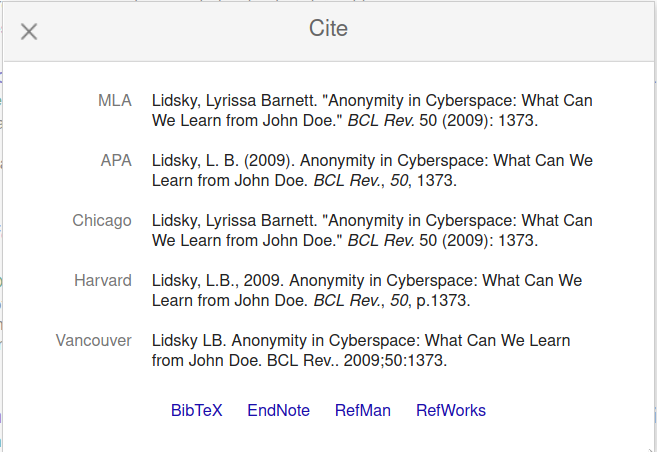
\includegraphics[scale=0.4]{./Pictures/Ilustracoes/2.png}
  \end{center}
  \legend{Fonte: o autor}
\end{figure}

Por fim, clicamos na opção BibTeX,
\begin{figure}[!htb]
  \caption{\label{im:3} Autogeração de meta-dados científicos}
  \begin{center}
    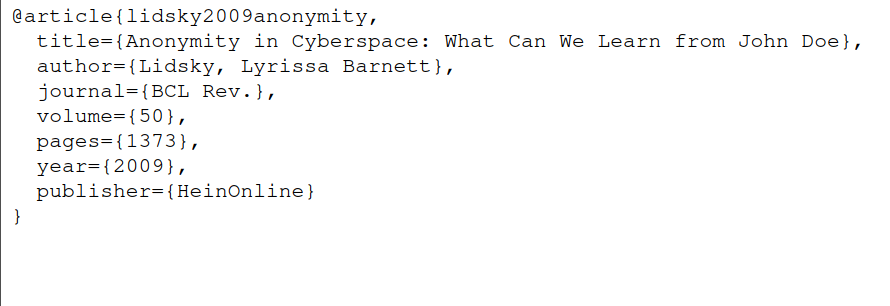
\includegraphics[scale=0.4]{./Pictures/Ilustracoes/3.png}
  \end{center}
  \legend{Fonte: o autor}
\end{figure}

\clearpage

\subsection{Citação textual}

Uma vez que temos os meta-dados em nosso arquivo .bib, armazenados,
utilizamos o primeiro argumento da lista de meta-dados, como argumento
da fução \verb+\cite{argumento-citação}+. Isto é, no caso da
\autoref{im:3}, para se fazer a citação textual, escreveríamos,
\verb_\cite{lidsky2009anonymity}_. O resultado que obteríamos é:
\cite{lidsky2009anonymity}.

Note que a formatação ABNT é seguida, com a classe abntex2. Se
utilizássemos a classe article, no entanto, essa formatação seria
diferente. %\footnote{mais inforamações na \autoref{sc:fmt}}

\subsection{Secção Bibliografia}

Para crearmos a citação bibliografia, utilizamos o comando
\verb_\bibliography{ref-bib}_. Desta forma, é formatada a secção
bibliográfica, a partir dos meta-dados .bib, sobreposto a estrutura que foi
modulada pela classe do documento (e.g., abntex2, article, book
etc).


\begin{figure}[!htb]
  \caption{\label{im:4} Secção Bibliográfica, classe abntex2}
  \begin{center}
    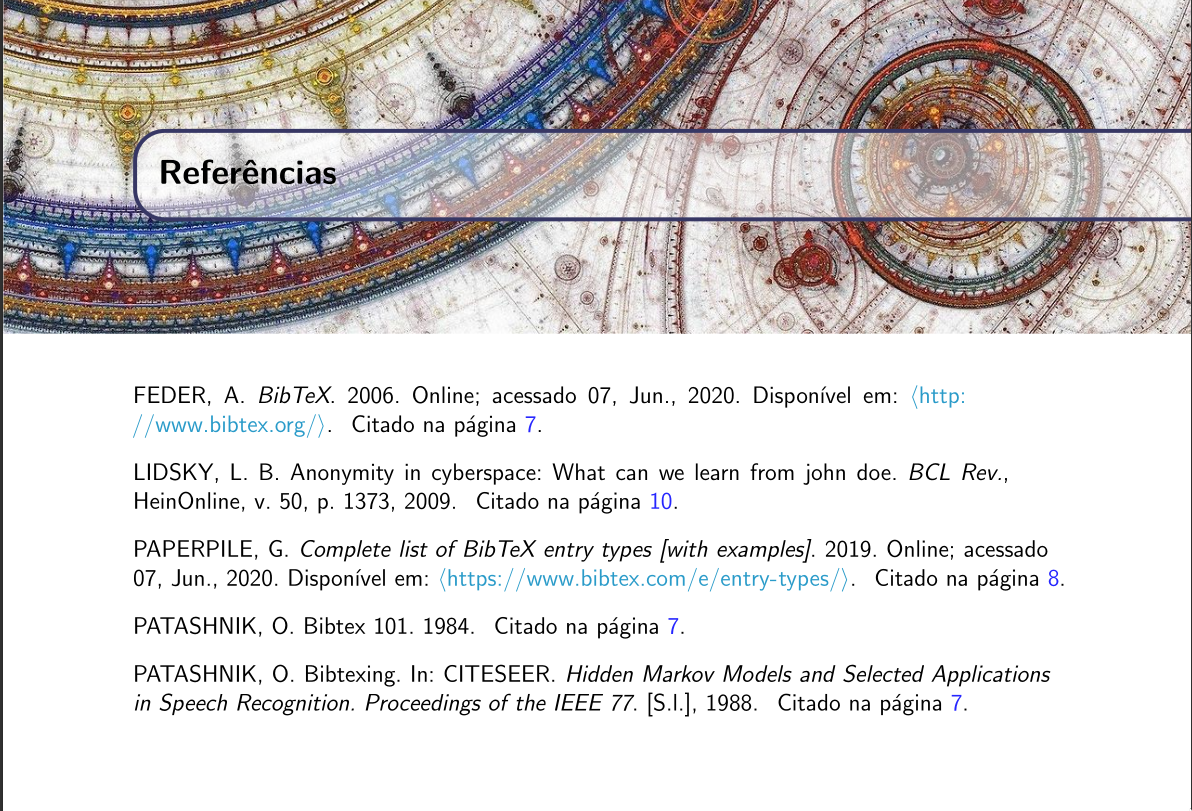
\includegraphics[width=\linewidth]{./Pictures/Ilustracoes/4.png}
  \end{center}
  \legend{Fonte: o autor}
\end{figure}

Felizmente, é possível, para citações sob a norma ABNT, puxar-se
um pacote separado da classe abntex2, \verb+\usepackage[alf]{abntex2cite}+.

\chapterimage{../bunnies.png}
\chapter{Apresentações}







  \begin{threeparttable}
    \begin{tabular}{rrrrrrrrr} \hline aaaaaaaa & aaaaaaaa & aaaaaaaa &
      aaaaaaaa & aaaaaaaa & aaaaaaaa & aaaaaaaa & aaaaaaaa &
      aaaaaaaa\\ \hline
    \end{tabular}%
    \begin{tablenotes}
    \end{tablenotes}
  \end{threeparttable}





\section{Classe Beamer}

A classe beamer é a mais utilizada para se fazer aprensentações, em
LaTeX. É possível, a partir de sua declaração, utilizar, já
estilizadas, opções de temas, cores e fontes.

\vspace{4mm}

Para tanto, precisamos declarar no preâmbulo os seguintes comandos,

\begin{itemize}
\item \verb+\usetheme{tema}+
\item \verb+\usecolortheme{cor-do-tema}+
\item \verb+\usefonttheme{font}+
\end{itemize}

\vspace{4mm}

As opções, nativas ao Beamer, possíveis são,

\begin{itemize}
\item \textbf{Temas}: AnnArbor Antibes Bergen Berkeley
Berlin Boadilla boxes CambridgeUS Copenhagen Darmstadt default Dresden
Frankfurt Goettingen Hannover Ilmenau JuanLesPins Luebeck Madrid
Malmoe Marburg Montpellier PaloAlto Pittsburgh Rochester Singapore
Szeged Warsaw.
\item \textbf{Cores}: albatross beaver beetle crane default dolphin dove fly lily
orchid rose seagull seahorse sidebartab structure whale wolverine.
\item \textbf{Fontes}: default professionalfonts serif structurebold
  structureitalicserif structuresmallcapsserif.
\end{itemize}

\vspace{4mm}

Claro que, podemos fazer todas as modulações que desejarmos, como
usualmente fazemos. Por exemplo, mudar a fonte da nossa apresentação
para Times, utilizando o pacote  ``times''.

\clearpage

\subsection{Estrutura da apresentação}

Todo slide é representado, dentro do LaTeX, por meio do ambiente
``frame''. Ademais, se quisermos que um mesmo slide tenha
comportamentos dinâmicos, como, por exemplo, itens aparecerem,
gradualmente, na tela, as modulações serão feitas dentro de um mesmo
ambiente-frame. Podemos ver isso pela comparação do código na
\autoref{im:5}, e o comportamento da mudaça de um ``slide'', da
\autoref{im:5} à \autoref{im:6}.

\begin{figure}[!htb]
  \caption{\label{im:5} Comparação do código e a apresentação}
  \begin{center}
    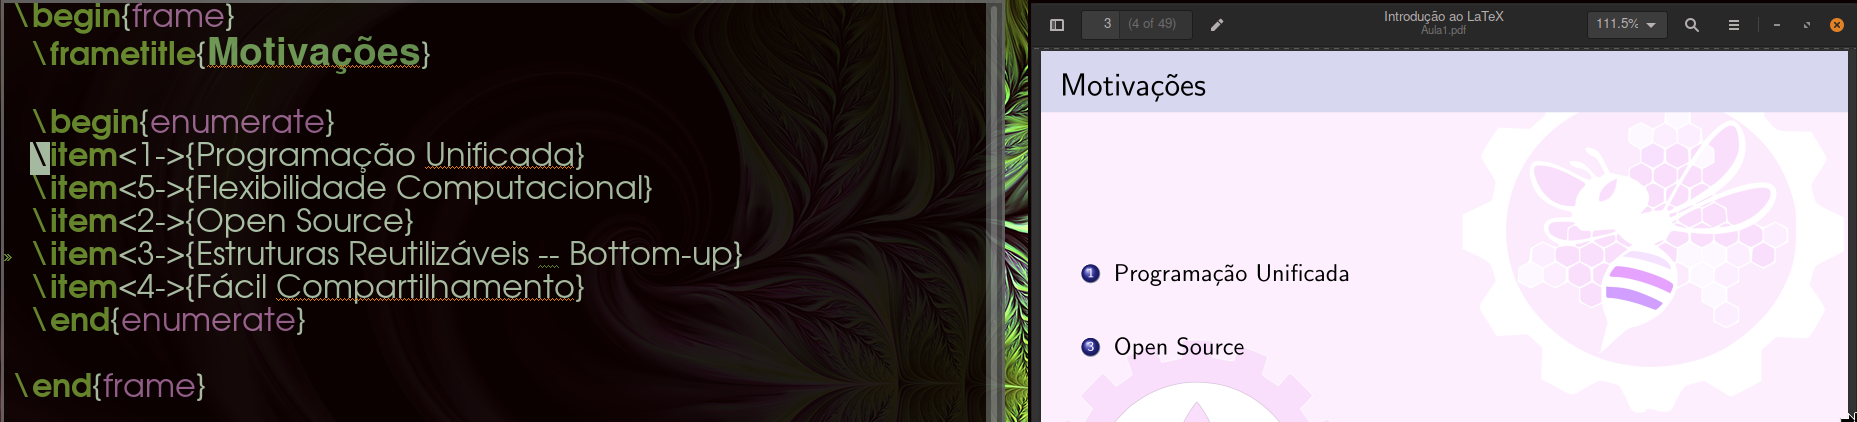
\includegraphics[width=\linewidth]{./Pictures/Ilustracoes/5.png}
  \end{center}
  \legend{Fonte: o autor}
\end{figure}

\begin{figure}[!htb]
  \caption{\label{im:6} Mudança de slide, no mesmo frame}
  \begin{center}
    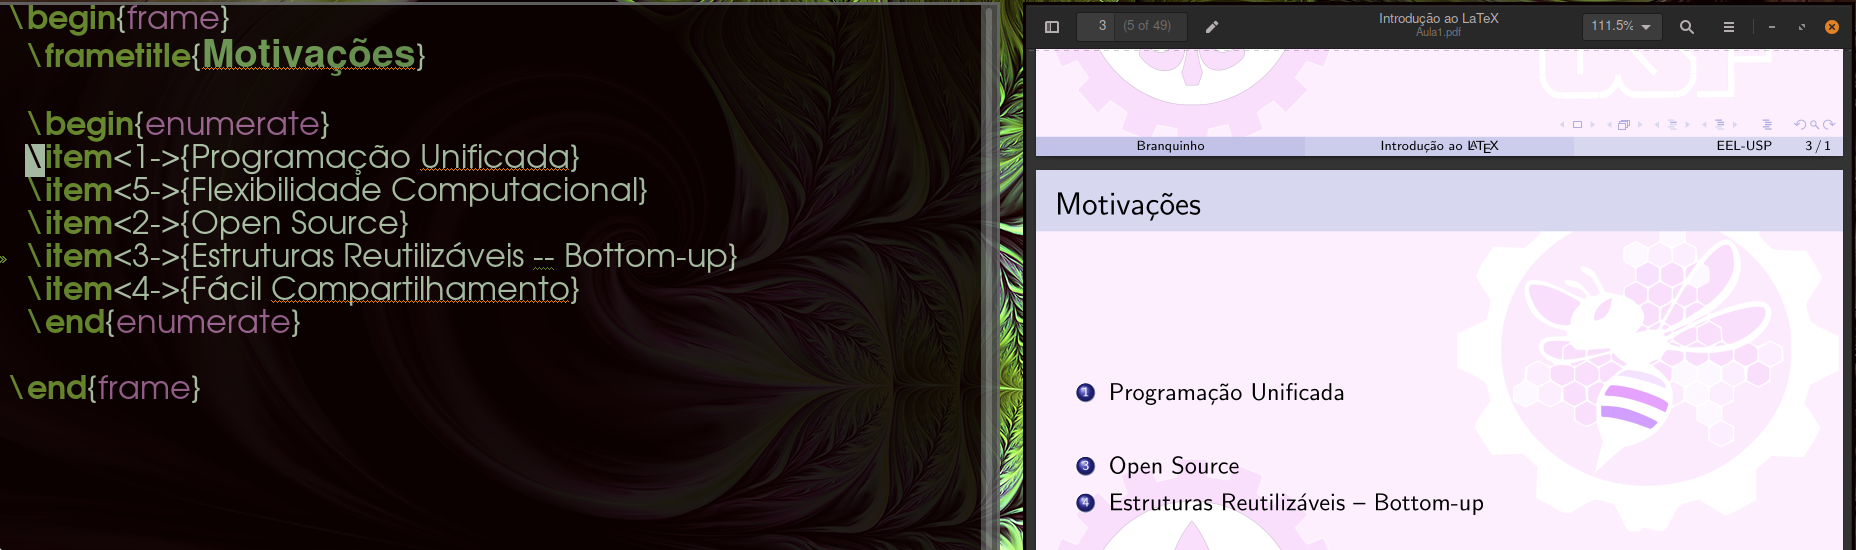
\includegraphics[width=\linewidth]{./Pictures/Ilustracoes/6.png}
  \end{center}
  \legend{Fonte: o autor}
\end{figure}

Note que podemos numerar em qual ordem, dos 5 slides, nesse caso
específico, que cada item aparecerá. Essa modulação também pode ser
feita com imagens, caixas e tabelas, utilizando as mesmas opções do itemize,
\verb+\comando<n-m>{}+. Isso faz com que o \emph{comando} apareça do slide
`n' ao slide `m'. se omitirmos um dos números, o comportamento se
estende, \verb+<n->+, do n até o fim do frame. Ou \verb+<-m>+ do início até o
m-ésimo slide do frame.

Portanto, um frame pode conter diversos slides. E, é possível crear
uma dinâmica dentro de uma sequência de slides de um mesmo frame.

\clearpage

\subsubsection{Ambiente caixa}

Nativamente, o Beamer diponibiliza comandos de caixas, eles são os
ambientes,
\begin{verbatim}
\begin{block}{nome-do-bloco}, \begin{alertbox}{nome} e \begin{examples}{nome}
\end{verbatim}

A munça de cada um deles é virtualmente
sua cor.

No entanto, existe um pacote, \verb+\usepackage{tcolorbox}+, o
qual capacita uma vasta gama de modulações a mais para
ambientes-caixas.

Fica aqui um exemplo utilizado na apresentação, \autoref{im:7},

\begin{figure}[!htb]
  \caption{\label{im:7} Comparação do código e a apresentação, pacote tcolorbox}
  \begin{center}
    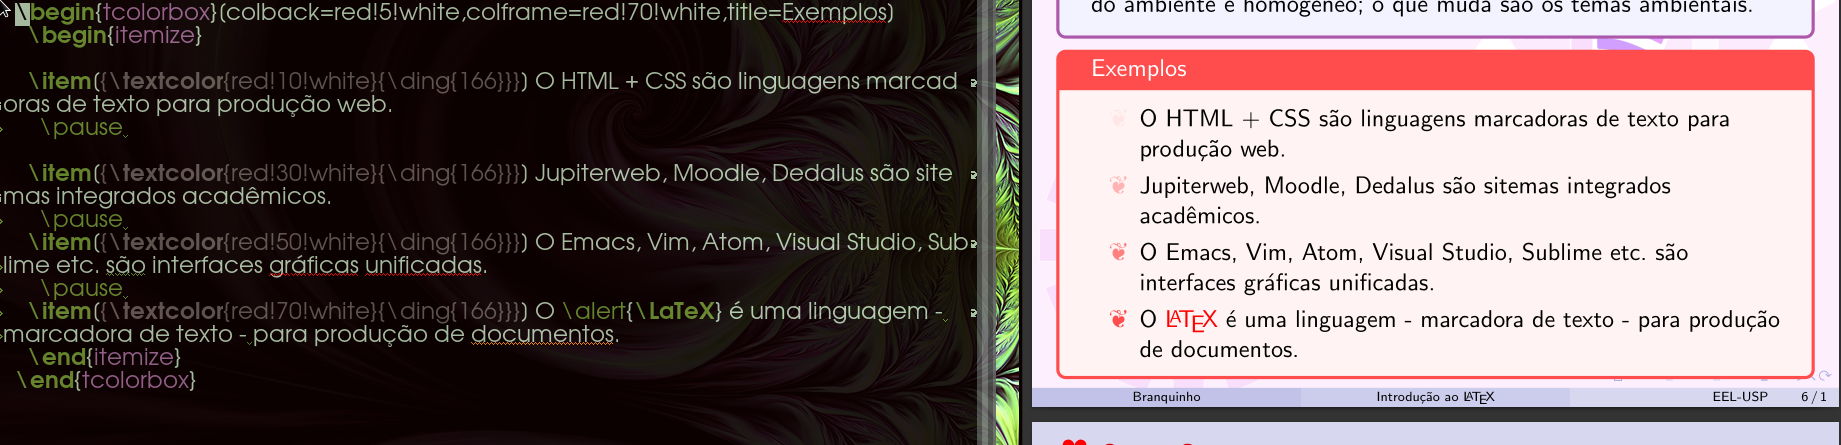
\includegraphics[width=\linewidth]{./Pictures/Ilustracoes/7.png}
  \end{center}
  \legend{Fonte: o autor}
\end{figure}


O código da \autoref{im:7}, é,

\begin{verbnobox}[\fontsize{12pt}{12pt}\selectfont]
\begin{tcolorbox}[colback=red!5!white,colframe=red!70!white,title=Exemplos]
  \begin{itemize}

  \item[{\textcolor{red!10!white}{\ding{166}}}] O HTML + CSS são
    linguagens marcadoras de texto para produção web.
    \pause

  \item[{\textcolor{red!30!white}{\ding{166}}}] Jupiterweb, Moodle,
    Dedalus são sitemas integrados acadêmicos.
    \pause
  \item[{\textcolor{red!50!white}{\ding{166}}}] O Emacs, Vim, Atom,
    Visual Studio, Sublime etc. são interfaces gráficas unificadas.
    \pause
  \item[{\textcolor{red!70!white}{\ding{166}}}] O \alert{\LaTeX} é uma
    linguagem - marcadora de texto - para produção de documentos.
  \end{itemize}
\end{tcolorbox}
\end{verbnobox}

\chapterimage{../25.jpg}
\chapter{Sumário de referências}
\vspace{1cm}

\section{Sites}

\begin{center}
\resizebox{0.90\textwidth}{!}{%



\begin{tcolorbox}[tabulars={@{\extracolsep{\fill}\hspace{1mm}}l|l|l@{\hspace{10mm}}},
  boxrule=0.5pt,title={\large \centering Sites de referência} \label{tab:sites}]

  \textbf{Comandos/Comportamentos} & \textbf{Pacotes} & \textbf{Sites} \\
  \hline \hline
  Matemática                             &  amsmath, esint &
  \href{http://linorg.usp.br/CTAN/macros/latex/required/amsmath/amsldoc.pdf}{amsmath},
  \href{http://linorg.usp.br/CTAN/macros/latex/contrib/esint/esint-doc.pdf}{esint}, \href{https://en.wikibooks.org/wiki/LaTeX/Mathematics}{wiki}  \\\hline
  Imagens, gráficos e cores             & tikz, graphicx, xcolors
  graphics   &
  \href{http://linorg.usp.br/CTAN/macros/latex/required/graphics/grfguide.pdf}{1},
  \href{http://linorg.usp.br/CTAN/info/epslatex/english/epslatex.pdf}{2},
  \href{https://en.wikibooks.org/wiki/LaTeX/PGF/TikZ}{wiki/tikz},
  \href{http://linorg.usp.br/CTAN/graphics/pgf/base/doc/pgfmanual.pdf}{tikz},
  \href{https://www.ctan.org/pkg/xcolor}{x}\\\hline
  ABNT                &  classe abntex, pacote abntex2cite
  & \href{https://www.ctan.org/pkg/abntex2}{doc. oficial (CTAN)} \\\hline
  Modelos & Overleaf, Repositórios &
  \href{https://github.com/26-55-87-BuddhiLW/MC-LaTeX}{Repositório},
  \href{https://www.overleaf.com/latex/templates}{Overleaf dasdsadas}\\\hline
  Apresentações & Beamer & \href{https://deic-web.uab.cat/~iblanes/beamer_gallery/index_by_theme.html}{Galeria}; \href{http://linorg.usp.br/CTAN/macros/latex/contrib/beamer/doc/beameruserguide.pdf}{docum.}
\end{tcolorbox}

}
\end{center}

Pode-se acessar uma lista completa de símbolos matemáticos
\href{https://www.caam.rice.edu/~heinken/latex/symbols.pdf}{aqui}. E,
lembre-se o \href{https://www.ctan.org/}{CTAN} sempre é mais extensa refência que você terá sobre
uma classe ou pacote. E, o \href{https://en.wikibooks.org/wiki/LaTeX}{wiki} também é uma fonte fantástica de informações

%%%%%%%%%% REFERÊNCIAS %%%%%%%%%%%%%%%%%%%
\chapterimage{../I9.jpg}
\bibliography{ref-bib}       %%puxa a bibliografia no diretório do
%% arquivo .tex, com nome 'ref-bib' (não
%% se põe se escreve a extensão .bib)



\end{document}

%%% Local Variables:
%%% mode: latex
%%% TeX-master: t
%%% End:
